\subsubsection{Implementacion 1}

\textbf{Explicacion Assembler}


En la primera implementación del filtro Merge, realizamos dos ciclos anidados los cuales iteran sobre la fila y sobre las columnas de la matriz de la imagen respectivamente. En el ciclo que itera sobre las columnas, iteramos de a cuatro píxeles, recorriendo toda una fila dictada por el otro ciclo. Estos punteros son iguales para ambas imagenes, dado que éstas tienen que ser de iguales dimensiones.

Al llegar al final de una fila, es decir, cuando el ciclo de las columnas termina, actualizamos los punteros de las imágenes sumándole al puntero el tamaño de la fila para cambiar a la siguiente, y realizamos las iteraciones hasta terminar de operar con todas las filas de la imagen.

\begin{figure}[ht!]
\centering
\includegraphics[width=90mm]{imagenes/merge/merge1_1.png}
\caption{*************INSERTAR IMAGEN DE UNA FILA RECORRIDA DENTRO DE LA MATRIZ*************
}
\end{figure}

Dentro del ciclo de las columnas guardamos en dos registros xmm los cuatro píxeles de cada imagen. Luego desempaquetamos cada registro en otros dos registros para incrementar el tamaño de las componentes de los pixeles y volvemos a repetir esta operacion para obtener cada pixel ocupando un registro xmm, una componente por doubleword, y así convertirlos a float.

%\begin{figure}[ht!]
%\centering
%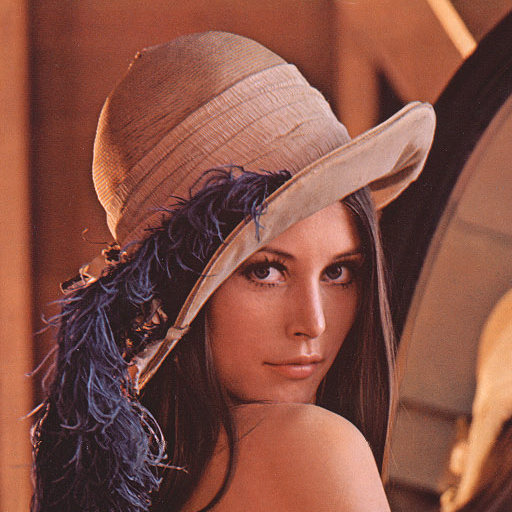
\includegraphics[width=90mm]{lena.bmp}
%\caption{*************INSERTAR IMAGEN DE LOS XMM CORRESPONDIENTES CON LAS LOS PIXELES*************}
%\end{figure}

Luego realizamos el producto del RGB del píxel por nuestro value, dejando intacto A, y al píxel ubicado en la misma posición pero en la otra imagen hacemos el producto por 1-value. A éstos valores los sumamos y convertimos estos valores a enteros, y los empaquetamos de dword a word y de word a byte para que el píxel recupere su valor original.

%\begin{figure}[ht!]
%\centering
%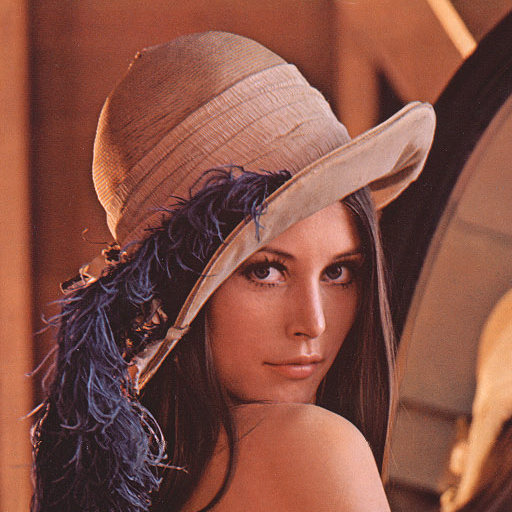
\includegraphics[width=90mm]{lena.bmp}
%\caption{*************INSERTAR IMAGEN DE LO QUE PASA CON RGB Y COMO EMPAQUETAMOS Y DESEMPAQUETAMOS*************
*}
%\end{figure}

Para finalizar, volvemos a guardar el pixel en memoria y termino de realizar la iteración, para volver a comenzar a repetir el proceso con los siguientes 4 píxeles

\subsubsection{Implementacion 2}

\textbf{Explicacion Assembler}


En la segunda implementación del filtro Merge se utiliza un ciclo, pero antes de inicializarlo, inicializamos un contador de filas y columnas , hacemos un Shuffle Packed Single(shufps) para tener 4 veces en el mismo registro el value y luego multiplicarle una máscara  para guardar v1 en un registro xmm y v2 en otro (convirtiéndolos a int previamente) y luego los empaquetamos para que sean int de 2 bytes.


\begin{figure}[ht!]
\centering
\includegraphics[width=90mm]{imagenes/merge/merge2_1.png}
\caption{***}
\end{figure}

Ya dentro del ciclo lo que se hace es copiar cuatro píxeles de cada imagen en dos registros xmm. Se utilizan dos registros xmm auxiliares en los cuales copiamos los píxeles y aplicando una mascara nos guardamos A ya que no debe ser modificado. Finalmente se desempaqueta y guardamos los píxeles en cuatro registros xmm (dos pixeles en cada uno).

\begin{figure}[ht!]
\centering
\includegraphics[width=90mm]{imagenes/merge/merge2_2.png}
\caption{***}
\end{figure}

Ahora comienza la parte de las operaciones, en la cual multiplicamos los registros de dos pixeles por v1 y realizamos lo mismo con esos registros por v2 guardándolos en otros registros. A continuación desempaquetamos para tener un pixel por registro, sumamos todos los xmm correspondientes y los dividimos por 256, los empaquetamos dos veces para que vuelvan a su tamaño original, aplicamos otra mascara para poner en 0 donde estaba el A modificado y luego reestablezco el A original de los píxeles que había guardado en el registro xmm auxiliar.

\begin{figure}[ht!]
\centering
\includegraphics[width=90mm]{imagenes/merge/merge2_3.png}
\caption{***}
\end{figure}

Luego de terminar con las operaciones, guardo en memoria los píxeles modificados avanzo el puntero 4 posiciones y me fijo si llego al final de la fila. En caso de llegar, Actualizo los punteros de las imágenes, avanzando una fila, reinicio el offset y avanzo el contador de filas, una vez que llego al final de las filas termino; si no terminé la fila vuelvo al ciclo y repito las operaciones con los píxeles siguientes.